\documentclass[11pt, oneside]{article}   	% use "amsart" instead of "article" for AMSLaTeX format
\usepackage[inner=1cm,outer=1cm]{geometry}              		% See geometry.pdf to learn the layout options. There are lots.
\geometry{letterpaper}                   		% ... or a4paper or a5paper or ... 
%\geometry{landscape}                		% Activate for rotated page geometry
%\usepackage[parfill]{parskip}    		% Activate to begin paragraphs with an empty line rather than an indent
\usepackage{graphicx}				% Use pdf, png, jpg, or eps§ with pdflatex; use eps in DVI mode
								% TeX will automatically convert eps --> pdf in pdflatex		
\usepackage{amssymb}
% PACKAGES FOR DRAWINGS
\usepackage{tikz}
\usetikzlibrary{shapes.geometric, arrows}
\tikzstyle{process} = [rectangle, minimum width=3em, minimum height=2em, text centered, draw=blue, fill=gray!10]
\tikzstyle{startend} = [ellipse, minimum width=2em, minimum height=1em, text centered, draw=red, fill=gray!10]
\tikzstyle{arrow} = [thick,->,>=stealth]
% COLOR FOR TABLES
\usepackage{colortbl} 
\usepackage{float}
\usepackage{verbatim}
\usepackage{enumitem}

%SetFonts

%SetFonts

\topmargin=-1 in
\textheight=10in

\title{A Model of College Admission Decision-Making Using Machine Learning}
\author{Kanadpriya Basu, Treena Basu, Ron Buckmire, Nishu Lal}
%\date{}							% Activate to display a given date or no date

\begin{document}
\maketitle



\section{Introduction}
\label{sec:intro}
Occidental College is a small, highly selective liberal arts college in North East Los Angeles with a mission ``to provide a gifted and diverse group of students with a total educational experience of the highest quality--one that prepares them for leadership in an increasingly complex, interdependent and pluralistic world." Each year the college receives an average of 6,292 applications of which around an average of 44\%  applicants are offered admission and an average of 535 students enroll.  

Occidental College collects various kinds of data about its admitted students such as Gender,  Ethnic Background, Top Academic Interest 
(categorical variables), First Generation to College and Campus Visit Indicator,  (binary variables), High School GPA, ACT score or SAT score (numerical variables) just to name a few. 


\section{Problem Statement}
\label{sec:problem statement}
With the four years of confidential data the college has provided about the annual admitted pool of students the goal of the project described in this paper is to make a prediction regarding each student and classify them into one of two categories: ``admitted student who will accept the admission offer" and ``admitted student who will reject the admission offer". In other words, we are working on a {\it binary classification problem} using {\it supervised machine learning} with the ultimate goal of being able to classify new instances, i.e. when we have a new admitted student we would like to able to predict whether or not that student will accept or reject the admission offer. 

Below in Figure \ref{fig:flowchart1} is a flowchart that represents the admission whittling process with the statistics for the classes of 2018 through 2021 (students admitted in 2014 through 2017):
%%----------------------------------------------------------
%%GRAPHICS: FLOWCHART
%%----------------------------------------------------------
\begin{figure}[H]
\centering
\hfill\\
{\scriptsize 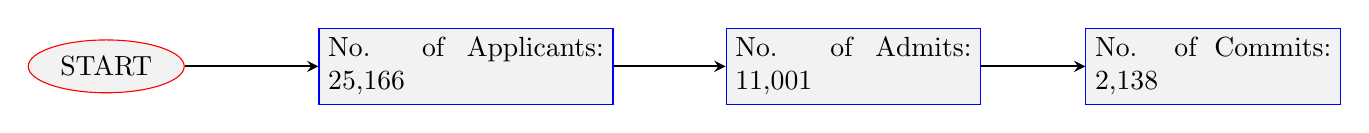
\begin{tikzpicture}[node distance=11em]

\node (S) [startend] {START};

\node (S1) [process, right of=S, xshift= 2em]{\parbox[t][][t]{3.5cm}{No. of Applicants: 25,166}};

\node (S2) [process, right of=S1, xshift=3em]{\parbox[t][][t]{3cm}{No. of Admits: 11,001}};

\node (S3) [process, right of=S2, xshift=2em]{\parbox[t][][t]{3cm}{No. of Commits: 2,138 }};

\draw [arrow] (S) -- (S1);
\draw [arrow] (S1) -- (S2);
\draw [arrow] (S2) -- (S3);
\end{tikzpicture}}
\caption{Summary Numbers for Class of 2018 through Class of 2021}
\label{fig:flowchart1}
\end{figure}
We will use the term `admits' to represent students whom the college has extended an admissions offer to and `commits' to represent the students who have accepted the offer. Note that  international students and early decision students have been omitted from our dataset and thus we have reduced our dataset from $11,001$ to $9,626$  admits.

The eight machine learning techniques implemented in this paper are: 
\begin{itemize}[noitemsep]
\item {\it Logistic Regression} (LG)
\item {\it Naive Bayes} (NB)
\item {\it Decision Trees} (DT)
\item {\it Support Vector Machine} (SVM)
\item {\it K-Nearest Neighbors} (kNN)
\item {\it Random Forests (RF)} (parallel ensemble), 
\item {\it Gradient Boosting} (GB) (sequential ensemble), 
\item and one deep learning technique: {\it Multi-Layer Perceptron (MLP)}
\end{itemize}

\section{The Data}
\label{sec:data}
Preprocessing is an important step in any data science project; the aim is to cleanse the dataset and prepare it to be further used in a prediction algorithm.
The confidential data received from Occidental College was organized and fairly clean and thus we needed to make only a few changes in order to make the data suitable for our chosen machine learning algorithms. 

The data consists of 36 pieces of personal information about admitted applicants.  Using these available features, our main task in this study will be to focus on the binary response of whether an admitted applicant to Occidental College will follow through on the offer, i.e., will they accept or reject the admission offer. 

A standard challenge in data cleaning is to determining how to deal with missing data. Simply disregarding data with missing entries results in loss of valuable information for the model to learn from and incorporating data with missing entries may compromise prediction results. It is important to identify the features with missing entries, locate such entries and implement some sort of treatment that allows us to incorporate the data into the model, since the feature in question may be a strong predictor in determining the algorithms outcome. For example, treatments may include replacing missing entries of a numerical variable with its median value and performing imputation technique to replace missing entries of categorical variables. The cleansing of the dataset results in $7,976$ admits.

Below in Table \ref{table:comparative statistics} we present the comparative statistics for the last four years starting from 2014 (Class of 2018) to 2017 (Class of 2021).
%%-------------------------------------------------------------------------------
%%TABLE: COMPARATIVE STATISTICS
%%-------------------------------------------------------------------------------
\begin{table}[H]
\caption{First-Year Commit Data (Raw)}
\label{table:comparative statistics}
\begin{center}
\begin{tabular}{ |c|c|c|c|c| } 
\hline
 & Class of 2018 & Class of 2019 & Class of 2020 & Class of 2021\\
 Applications &  & & & \\
\hline
Number of Applicants  & 6,071 & 5,911 & 6,409 & 6,775 \\  \hline
Admit Number and Admit \% & 2,549, 42\% & 2,659, 45\% & 2,948, 46\% & 2,845, 42\%  \\ \hline
Number Enrolled  and Enrolled \% & 547, 9.01\% & 518, 8.76\% & 502, 7.83\% & 571, 8.42\%\\
\hline
\end{tabular}
\end{center}
\end{table}
We observe and address the inherent class imbalance of this dataset. Since only 17\% of all admits accept the admission offer (as calculated from the cleansed dataset), simply using the {\it accuracy} score could result in a false impression regarding the model performance. Instead we use the more suitable metrics of {\it precision, recall, $F_\beta$ score} and {\it area under the receiver operator curve} to overcome the challenges caused by class imbalance.

\section{Prediction Techniques}
\label{sec:summary of classification techniques}
The goal of this paper is to compare the eight classification techniques in the context of college commitment of admitted students. Below in Flowchart \ref{fig:workflow} we illustrate the main steps executed to arrive at a prediction of a new instance.
%%----------------------------------------------------------
%%GRAPHICS: WORKFLOW
%%----------------------------------------------------------
\begin{figure}[H]
\centering
\hfill\\
{\scriptsize 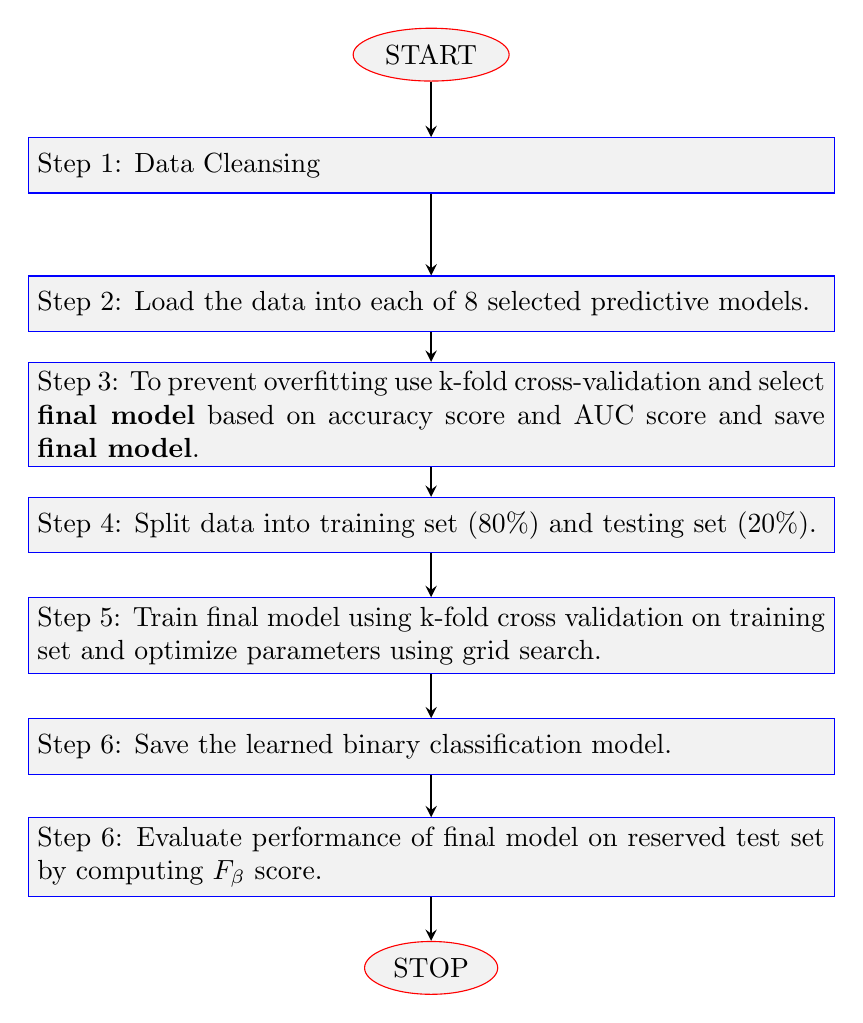
\begin{tikzpicture}[node distance=2em]

\node (S) [startend] {START};

\node (S1) [process, below of=S, yshift= -2em]{\parbox[t][][t]{10cm}{Step 1: Data Cleansing}};

\node (S2) [process, below of=S1, yshift=-3em]{\parbox[t][][t]{10cm}{Step 2: Load the data into each of 8 selected predictive models.}};

\node (S3) [process, below of=S2, yshift=-2em]{\parbox[t][][t]{10cm}{Step 3: To prevent overfitting use k-fold cross-validation and select {\bf final model} based on accuracy score and AUC score and save {\bf final model}.}};

\node (S4) [process, below of=S3, yshift=-2em]{\parbox[t][][t]{10cm}{Step 4: Split data into training set (80\%) and testing set (20\%).}};

\node (S5) [process, below of=S4, yshift=-2em]{\parbox[t][][t]{10cm}{Step 5: Train final model using k-fold cross validation on training set and optimize parameters using grid search.}};

\node (S6) [process, below of=S5, yshift=-2em]{\parbox[t][][t]{10cm}{Step 6: Save the learned binary classification model.}};

\node (S7) [process, below of=S6, yshift=-2em]{\parbox[t][][t]{10cm}{Step 6: Evaluate performance of final model on reserved test set by computing $F_\beta$ score.}};

\node (S8) [startend, below of=S7, yshift=-2em]{STOP};

\draw [arrow] (S) -- (S1);
\draw [arrow] (S1) -- (S2);
\draw [arrow] (S2) -- (S3);
\draw [arrow] (S3) -- (S4);
\draw [arrow] (S4) -- (S5);
\draw [arrow] (S5) -- (S6);
\draw [arrow] (S6) -- (S7);
\draw [arrow] (S7) -- (S8);

\end{tikzpicture}}
\caption{Workflow}
\label{fig:workflow}
\end{figure}

\section{Conclusions and Future Work}
\label{sec:conclusions and future work}
Our studies indicate promising results for the role of supervised machine learning algorithms in determining student outcomes in the college admission process. This paper analyzed and compared the results of applying eight classifiers to a data set containing $7,976$ samples representing 
admitted applicants to Occidental College and their personal attributes. Each prediction technique was trained on the entire data set,
and their performance was measured by calculating the accuracy and AUC score through k-fold cross validation. The model with the best AUC score (Logistic Regression) was then selected. To measure the effectiveness of the best model, we divide the data into two parts, and train the model on 80\% of the data and finally test it on 20\% of the data that was held out. Finally, we optimize the performance of the final model with grid search technique.  

We conclude this section with a discussion about some avenues for future research in this area as a result of these findings. 
Firstly, ``better and cleaner data" often beats better algorithms, and designing good features goes a long way so an aspect to consider is how to
collect ``better and cleaner data", i.e., collect data on features that have more predictive powers than the features we had for this study. This is a difficult question that may require deep knowledge of the problem domain.
This might be achieved by designing arrival surveys for incoming students to better understand their reasons for committing to
the college. Another approach may be to establish a pipeline for collaborative research between local and district schools with institutions of higher education to detect the extent of college intentions of graduating students. Further studies on feature selection could result in simplification of models and shorter training times in some cases.

\section{The Impact of this Research}
The future and sustainability of the traditional higher education business model is up for much debate recently, especially with rising costs of tuition, concerns about the debt incurred by students and their family, unsure job prospects and the availability of cheaper options to specialized education such as massive open online courses (MOOCs) \cite{tiaacref}.

This business model is of course highly dependent on the type of academic institution being considered, such as public colleges and universities, private non-profit colleges and private for-profit colleges.
Primary sources of income for institutes of higher education include: student tuition, government funding, endowments, alumni donations and fees-for-service. In order to ensure financial stability, many colleges and universities are  trying to operate at full capacity which means 
increasing their target enrollment.

The cost (sticker price) of attending a small liberal arts college such as Occidental College is \$70,182 for the 2018-2019 academic year \cite{Oxy}. If the college falls below its target enrollment by only 10 students this could result in a potential financial loss of \$701,820 per year for four years, amounting to a total loss of more than \$2.8 million. The reader should note that this only represents a potential financial loss and that some students receive a discount rate. However, this discount rate is not determined until after a student has enrolled.
\begin{comment}
{\bf\color{red} The problem with this prior statement is that the sticker price of  a College is not the actual amount of money they bring in--that's why there is something called the ``discount rate." This is the percentage of the tuition that is actually paid by he average student. I believe Oxy's discount rate is around 34\%.}
\end{comment}
Not to mention the loss of future revenue that these admitted students who don't attend could have generated through alumni donations. Thus, it is very important for an academic institution to definitively know how many incoming students they can expect to enroll, especially if they are relying on the revenue generated from the tuition the students bring in. 
%Please note "institute" should be changed to "institution" wherever it appears, unless its being used as a verb.

The authors acknowledge that data science has not been used very often in the academic business model of determining whether a student will accept or reject an admissions offer. The mathematical model developed in this paper  simply requires knowledge of personal traits of individual applicants so that it can be fed into the applied algorithms. Being able to accurately predict whether or not a student admitted to an academic institute will accept or reject the admissions offer can help institutions of higher education reach target enrollment. For many institutions, enrollment management is a key component of academic administration.

For example, suppose the model predicts an applicant will reject the admissions offer. Under these circumstances the institution can focus on increasing communications (e.g.through emails, texts and counseling) with such individuals and perhaps allocate resources to provide them the support they need to help make a decision. Or, alternatively, if our model predicts certain students will accept an offer of admission  then the admissions office  can focus resources on recruiting these students to actually attend. In the parlance of admissions, this is known as increasing the yield rate of admitted students.

%\item Widen the perspective pool of students if enough are not found from the usual target audience, i.e., instead of focusing on simply the 
%traditional student audience one could target a variety of audiences such as veterans, international students along with older students.

\begin{thebibliography}{00}

%%Textbooks 
\begin{comment}
\bibitem{Godsey} Brian Godsey, 
Think Like a Data Scientist {\em Manning}, ISBN: 9781633430273 

\bibitem{BrRiFe} H.~Brink, J.~Richards, M.~Fetherolf, Real World Machine Learning,
 {\em Manning}, ISBN: 9781617291920

\bibitem{CiMeAl} D.~Cielen, A.~Meysman, M.~Ali,
Introducing Data Science, {\em
Manning} ISBN: 9781633430037.

\bibitem{Gr} J.~Grus, Data Science From Scratch First Principles With Python, {\em O'Reilly} 
ISBN: 9781491901427

\bibitem{Ge} A.~G\'{e}ron, Hands-On Machine Learning with Scikit-Learn \& Tensor Flow, {\em O'Reilly} 
ISBN: 9781491962299

\bibitem{HaTiFr} T.~Hastie, R.~Tibshirani, J.~Friedman, The Elements of Statistical Learning, Second Edition, {\em Springer} 

\bibitem{JaWiHaTi} G.~James, D.~Witten, T.~Hastie, R.~Tibshirani, An Introduction to Statistical Learning with Applications in R, {\em Springer}, ISBN 9781461471370
\end{comment}
%%Papers
\bibitem{tiaacref} L.~Lapovsky, TIAA-CREF Institute, The Higher Education Business Model,
Innovation and Financial Sustainability.
https://www.tiaa.org/public/pdf/higher-education-business-model.pdf

\bibitem{Oxy} https://www.oxy.edu/admission-aid/costs-financial-aid

%\item https://fivethirtyeight.com/features/fancy-dorms-arent-the-main-reason-tuition-is-skyrocketing/
\end{thebibliography}
\end{document}  